% do not change these two lines (this is a hard requirement
% there is one exception: you might replace oneside by twoside in case you deliver 
% the printed version in the accordant format
\documentclass[11pt,titlepage,oneside,openany]{article}
\usepackage{times}


\usepackage{graphicx}
\usepackage{latexsym}
\usepackage{amsmath}
\usepackage{amssymb}
\usepackage[utf8]{inputenc}
\usepackage{ntheorem}

% \usepackage{paralist}
\usepackage{tabularx}

% this packaes are useful for nice algorithms
\usepackage{algorithm}
\usepackage{algorithmic}

% well, when your work is concerned with definitions, proposition and so on, we suggest this
% feel free to add Corrolary, Theorem or whatever you need
\newtheorem{definition}{Definition}
\newtheorem{proposition}{Proposition}


% its always useful to have some shortcuts (some are specific for algorithms
% if you do not like your formating you can change it here (instead of scanning through the whole text)
\renewcommand{\algorithmiccomment}[1]{\ensuremath{\rhd} \textit{#1}}
\def\MYCALL#1#2{{\small\textsc{#1}}(\textup{#2})}
\def\MYSET#1{\scshape{#1}}
\def\MYAND{\textbf{ and }}
\def\MYOR{\textbf{ or }}
\def\MYNOT{\textbf{ not }}
\def\MYTHROW{\textbf{ throw }}
\def\MYBREAK{\textbf{break }}
\def\MYEXCEPT#1{\scshape{#1}}
\def\MYTO{\textbf{ to }}
\def\MYNIL{\textsc{Nil}}
\def\MYUNKNOWN{ unknown }
% simple stuff (not all of this is used in this examples thesis
\def\INT{{\mathcal I}} % interpretation
\def\ONT{{\mathcal O}} % ontology
\def\SEM{{\mathcal S}} % alignment semantic
\def\ALI{{\mathcal A}} % alignment
\def\USE{{\mathcal U}} % set of unsatisfiable entities
\def\CON{{\mathcal C}} % conflict set
\def\DIA{\Delta} % diagnosis
% mups and mips
\def\MUP{{\mathcal M}} % ontology
\def\MIP{{\mathcal M}} % ontology
% distributed and local entities
\newcommand{\cc}[2]{\mathit{#1}\hspace{-1pt} \# \hspace{-1pt} \mathit{#2}}
\newcommand{\cx}[1]{\mathit{#1}}
% complex stuff
\def\MER#1#2#3#4{#1 \cup_{#3}^{#2} #4} % merged ontology
\def\MUPALL#1#2#3#4#5{\textit{MUPS}_{#1}\left(#2, #3, #4, #5\right)} % the set of all mups for some concept
\def\MIPALL#1#2{\textit{MIPS}_{#1}\left(#2\right)} % the set of all mips





\begin{document}

\pagenumbering{roman}
% lets go for the title page, something like this should be okay
\begin{titlepage}
	\vspace*{2cm}
  \begin{center}
   {\Large Information Retrieval Project Report \\}
   \vspace{2cm} 
   {Class Project\\}
   \vspace{2cm}
   {presented by\\
    Michael Dell(1359533), Alexander Müller(1376818), Maxim TODO  \\
    
   }
   \vspace{1cm} 
   {
    University Mannheim\\} \vspace{2cm}
   {July 2014}
  \end{center}
\end{titlepage} 

% no lets make some add some table of contents
%\tableofcontents
\newpage

%\listofalgorithms

%\listoffigures

%\listoftables

% evntuelly you might add something like this
% \listtheorems{definition}
% \listtheorems{proposition}

\newpage


% okay, start new numbering ... here is where it really starts
\pagenumbering{arabic}
\section{Introduction and Problem Statement}
Maxim
\section{Architecture Overview}
Michi
\section{Extraction Pipeline}
\section{HTML Extraction}
Michi
\subsection{Person Contact Information Extraction}

TODO Michi

After we exploited the structure of the website, the need of having additional checks whether the heuristic really extracted a person or not came up. Therefore we decided to make use of Name Entity Recognition (NER). NER is defined as the identification of proper names in text or collection of text and assign them to a category person, location and organization. Due to our problem domain we only considered Named Entities (NE) of the type Person. 

A well-known library for Natural Lange Processing (NLP) tasks is Stanford Core NLP \cite{manning2014}, which also includes in their current version a NER Component to recognize English names. Of course this is not optimal and therefore we combined the current version of Stanford Core NLP with an older where a German NER Component exists \cite{faruqui10}. 

In the evaluation Chapter we will investigate how this two different libraries performed. 

Consequently we used for our purposes both NER Components in combination. As illustrated above we exploit the html structure of a webpage. Therefore we iterate over the DOM Structure and only consider header elements. If in one heading, one of the NER Components finds a NE of type Person, the algorithm tries to extract contact information in the corresponding parts of the html documents, otherwise it continues.

The result of this step of our pipeline is a set of person entity candidates that still can contain corrupt or duplicate data. Therefore the next step is to clean the set.
\subsection{Candidate Pruning}
The person entities extracted in the previous step of the extraction pipeline can still contain a lot of corrupt data.  Some examples are extractions that relate to a NE in the heading, but no contact data in the related parts like: “Publications of Prof. Dir. Simone Paolo Ponzetto”. Furthermore there will be a lot of duplicates in the resulting set, because lots of university employees do have their contact data on duplicate webpages.

To solve the first case we once more analyze the heading that lead to the extraction of contact data and count how many of the words are on a name word list. If this is more than one third we consider them this as a correctly extracted Person entity. 

Second to eliminate duplicate entries we developed a light-weight heuristic to identify them. For the ease of use we define that two people are duplicate entities when first name, last name and the email address are the same. Now the question arose which one to keep? For further improving the performance of our system we decided to keep the entity with most not null values in its fields.

After this step the set of candidate entities was pruned in order to assure a high data quality.
\subsection{Enable Search with Apache Solr}

In the previous chapters the extraction of person entities associated with their contact data was presented. In order to make this information accessible to end-users, to fulfill their information need an information retrieval system is necessary. A special requirement is fulfilling the need of field queries for the purpose of inverse searches. For instance if a user got a call from a telephone number he doesn't know, he want to retrieve all people that have the corresponding number.

An ideal system to fulfill those user requirements is Apache Solr, which was developed as all-in-one information retrieval/search engine. It fulfills the tasks of index creation, both for free-text queries and field search, as well as the handling and parsing of user queries.  Since our problem the search problem in our case is not an typical search on unstructured or semi-structured data residing in textual documents we need to change the configuration of Apache Solr.

\begin{figure}
  \begin{center}
   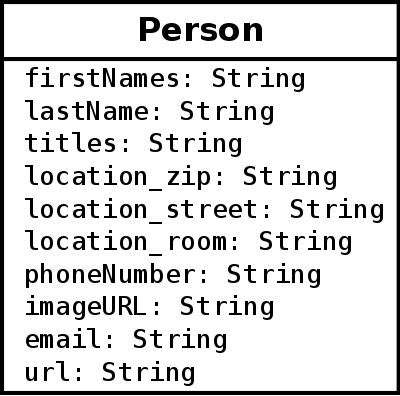
\includegraphics[width=0.38\textwidth]{figures/Person.png}
  \end{center}
  \caption{Datastructure of a Person Entity}
    \label{fig:person}
\end{figure}

The entities that were extracted are stored in a MySQL database with the representation as shown in Figure \ref{fig:person}.  In order to allow Solr to access the database we needed to change some of the configuration parameters. First of all necessary java classed needed to be included to allow Solr to establish a JDBC connection to the database the entities reside in. Now we enabled the creation of inverted indices both, for field queries and free text queries considering all fields when the user enters his or her query. 

This query interface is in Apache Solr by default exposed via webservices, which we used to communicate to our custom build User Interface which will be described in the following section.
\subsection{User Interface}
TODO Michi
\section{Project Evaluation}
Maxim
\section{Summary}
Maxim
%\bibliographystyle{plain}
%\bibliography{thesis-ref}


%\appendix



\newpage



\bibliographystyle{plain}
\bibliography{thesis-ref}


\end{document}
